\documentclass{scrartcl}

\usepackage{fontenc}
\usepackage[english]{babel}
%%\usepackage{ulem}
\usepackage{blindtext}
\usepackage{parskip}

\usepackage{amsmath}

\usepackage{graphicx}

\setlength{\parindent}{0pt}

\usepackage[style=apa, backend=biber, natbib=true, bibencoding=utf8]{biblatex}

\addbibresource{gesis_panel_bibliography.bib}




\title{Spielerei}
\author{Bernd Weiß}
\date{\today}

\begin{document}

\maketitle

\tableofcontents

%\chapter{erstes kapitel \$}


siehe abbildung~\ref{fig:histogram} in abschnitt~\ref{sec:eins}

	das ist ein test

\texttt{das ist schreibmaschinentext}	

	\today
	
\input{input-ex.inc}

\section{zweiter teil}

\section{erster teil}\label{sec:eins}

\subsection{erster unterabschnitt}

\begin{figure}
    \centering
        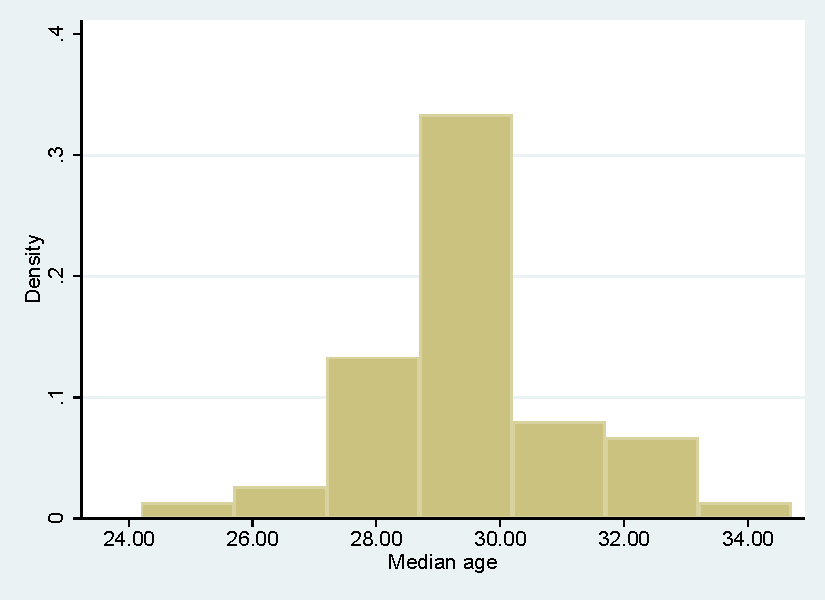
\includegraphics[width= 0.8\textwidth]{hist-plot-age.pdf}
    \caption{Ein ganz wunderbares histogram}
    \label{fig:histogram}
\end{figure}


\begin{table}[]
\begin{tabular}{lllll}
12 & 3 & 7 & 7 &  \\
7  & 7 & 7 &   &  \\
7  & 5 & 7 & 7 &  \\
   &   &   &   & 
\end{tabular}
\end{table}

\vspace{2ex}

\begin{table}	
\caption{meine tabelle}\label{tab:meine-tabelle}
\centering
\begin{tabular}{|cc}
    \hline
	1.1666666 & 1.2 \\
	2.1 & 2.2 \\
\end{tabular}	
\end{table}

\emph{dies \emph{ist} ein text}

\mdseries

%%ein tolles zeichen ist \[\alpha_1^{\beta_1}\].

\begin{equation*}
    \alpha_1^{\beta_1}
\end{equation*}

\clearpage

\begin{itemize}
    \item eins
    \item zwei
    \item drei
\end{itemize}

\begin{enumerate}
    \item eins
    \item zwei
    \item drei
\end{enumerate}

\begin{description}
    \item[Schlagwörter] stehen
    am Anfang einer Zeile und
    werden jeweils fett gedruckt,
    während die zugehörige \ldots
    \item[Beschreibung]
    dahinter in normaler Schrift
    erscheint. 
\end{description}


dies test relativ langweilig dies test relativ langweilig dies test relativ langweilig dies test relativ langweilig dies test relativ langweilig dies test relativ langweilig dies test relativ langweilig dies test relativ langweilig dies test relativ langweilig dies test relativ langweilig dies test relativ langweilig dies test relativ langweilig 

\noindent dies test relativ langweilig dies test relativ langweilig dies test relativ langweilig dies test relativ langweilig dies test relativ langweilig dies test relativ langweilig dies test relativ langweilig dies test relativ langweilig dies test relativ langweilig dies test relativ langweilig dies test relativ langweilig dies test relativ langweilig 


\begin{flushleft}
\blindtext[5]
\end{flushleft}

\textbf{das ist durchgestrichen}
	
\citet[456]{schaurerInvestigatingSelectionBias2020} sagen, alle online-forschung ist biased! onlineforschung	wird die welt beherrschen \citep[siehe bspw.][789]{ackermannStealthDemocracyErklaerende2018a,  gutfleischPerceptionsSocietyNecessary2020, bosnjakEstablishingOpenProbabilityBased2018}
	
\parencites[vgl.][1]{ackermannStealthDemocracyErklaerende2018a,  [siehe.][1]gutfleischPerceptionsSocietyNecessary2020, [vgl.][123]bosnjakEstablishingOpenProbabilityBased2018}	

\parencites[vgl.][1-2]{ackermannStealthDemocracyErklaerende2018a}[vgl.][3-4]{gutfleischPerceptionsSocietyNecessary2020}[vgl.][5-6]{bosnjakEstablishingOpenProbabilityBased2018}
	
\printbibliography	
	
\end{document}

